\begin{figure*}[!t]
  \centering
  \includegraphics[width=0.75\textwidth]{figures/LP-FLARE-polytope-5at-10x.pdf}
  \caption{Activation-feasible compositions from the LP screen, projected onto the
eleven-element composition simplex. The left panel shows the \(10\times\)W
feasible region, and the right panel the \(10\times\)EUROFER97 region, with feasible
compositions as points and the projected vertex hull outlined.}
  \label{fig:polytope}
\end{figure*}

\section{Results and Discussion}
\label{sec:results}

\subsection{Activation-Feasible Space}
\label{subsec:feasible}
The \(5\)~at.\% grid of the eleven-element system contains \(30{,}045{,}015\)
compositions. The LP construction identifies \(210\) of them as feasible under the
\(10\times\)W reference and \(61{,}297\) under the \(10\times\)EUROFER97 reference
(Fig.~\ref{fig:polytope}), the two sets corresponding to the plasma-facing and
structural sides of the wall. The difference of more than two orders of magnitude
reflects the lower activation of pure W, for which ten times the baseline is the
tighter bound. Although all eleven elements were free to vary, Ta, Nb, Mo, and Hf do
not occur in either set: they are excluded by activation alone, before any property
is considered. Every composition retained here, and therefore every layer of the
final gradient, stays within a factor of ten of its reference material for all
activation responses under the conditions of Table~\ref{tab:ind_variables}.

The LP construction returned exactly the compositions found by brute-force FLARE
evaluation of the full grid, with every response agreeing to numerical precision,
at a fraction of the cost (Table~\ref{tab:benchmark}). Brute force evaluates all
\(30{,}045{,}015\) grid compositions, whereas the LP approach evaluates only those
inside the polytope, reducing the wall-clock time from
\textcolor{red}{[\,\(t_{\mathrm{BF}}\)\,]} to \textcolor{red}{[\,\(t_{\mathrm{LP}}\)\,]}
and the peak memory from \textcolor{red}{[\,\(m_{\mathrm{BF}}\)\,]} to
\textcolor{red}{[\,\(m_{\mathrm{LP}}\)\,]}. The brute-force cost grows with the number
of grid points, which increases combinatorially with the number of elements and the
grid resolution, while the LP cost grows with the size of the feasible set, so the
advantage widens as the design space is refined.

\begin{table}[H]
\centering
\caption{Cost of identifying the activation-feasible compositions by brute-force
evaluation and by the LP construction, for both references. Hardware and software
are given in Section~\ref{sec:feasible-space}.}
\label{tab:benchmark}
\begin{tabularx}{\columnwidth}{lXX}
\toprule
 & Brute force & LP \\
\midrule
Compositions evaluated       & \(30{,}045{,}015\) & \textcolor{red}{[\,\,]} \\
Feasible, \(10\times\)W        & \(210\)            & \(210\) \\
Feasible, \(10\times\)EUROFER97 & \(61{,}297\)      & \(61{,}297\) \\
Wall-clock time              & \textcolor{red}{[\,\,]} & \textcolor{red}{[\,\,]} \\
CPU cores used               & \textcolor{red}{[\,\,]} & \textcolor{red}{[\,\,]} \\
Peak memory                  & \textcolor{red}{[\,\,]} & \textcolor{red}{[\,\,]} \\
Speed-up                     & \(1\times\)        & \textcolor{red}{[\,\,]} \\
\bottomrule
\end{tabularx}
\end{table}


\subsection{Phase Stability, Thermal Conductivity, and the Design Region}
\label{subsec:subgraphs}

Merging the two activation-feasible sets, in which \(204\) compositions are feasible
under both references, gives \(61{,}303\) unique compositions. Of these, \(700\)
(\(1.1\%\)) satisfy the phase-stability and conductivity criteria of
\Cref{eq:filters}. Phase stability is the decisive filter: \(50{,}365\) compositions
conduct heat adequately, but only \(706\) remain single-phase BCC at all three
temperatures. The reduced-activation space is therefore dominated by compositions
that would form intermetallics in service, and a gradient designed without a phase
constraint would almost certainly pass through them.

On the composition graph, the \(700\) compositions form three disconnected subgraphs
(Fig.~\ref{fig:clusters}). Subgraph~1 holds \(686\) compositions, \(98\%\) of the
total, extending from the tungsten-rich corner through the vanadium- and
titanium-rich region toward chromium. Subgraphs~2 and~3 are islands of eight and six
compositions, near the Fe corner and in the interior of the simplex, that satisfy
every screen yet cannot be reached from Subgraph~1 without passing through a
composition that fails one. Subgraph~1 is the only region in which a gradient can be
built from feasible layers alone, and it is the design region.

\begin{figure}[H]
  \centering
  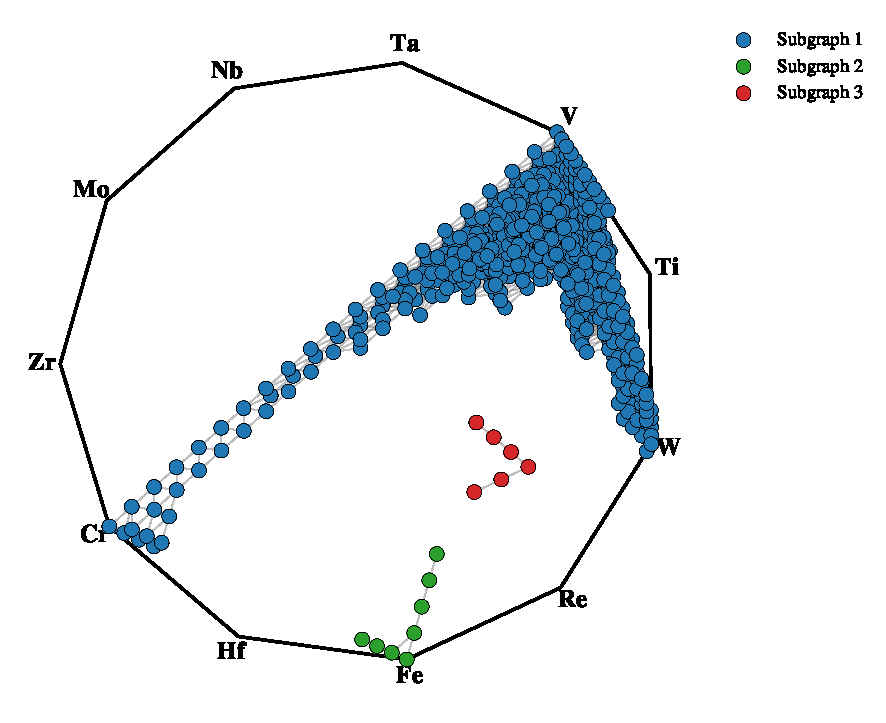
\includegraphics[width=0.75\linewidth]{figures/fig1_subgraphs.pdf}
  \caption{Connected subgraphs of the \(700\) compositions that pass the
  activation, single-phase BCC, and thermal-conductivity screens, projected onto
  the eleven-element composition space, with each element at a vertex. Circled
  numbers identify the subgraphs: Subgraph~1 (blue, \(686\) compositions) is the
  design region, and Subgraphs~2 (green) and~3 (red) are isolated islands of eight
  and six compositions.}
  \label{fig:clusters}
\end{figure}


\subsection{Plasma-Facing and Structural Materials}
\label{subsec:classification}

Classifying the design region by the two sides of the wall (\Cref{eq:classes})
gives \(139\) plasma-facing compositions (Material~A), \(169\) structural
compositions (Material~B), and \(18\) that qualify for both (Material~AB); the
remaining \(360\) are Intermediate (Fig.~\ref{fig:categories}). The two materials
occupy opposite ends of the design region, Material~A the tungsten-rich corner and
Material~B the vanadium-rich region, with Material~AB between them, where high
melting point and ductility coexist. Of the Intermediate compositions, \(193\)
satisfy the melting or ductility criterion but fall below the EUROFER97-level
strength, and \(184\) of these are ductile, vanadium-rich compositions that are too
weak at \(650^{\circ}\)C. The strength requirement therefore limits chiefly the
structural side of the wall.

\begin{figure}[H]
  \centering
  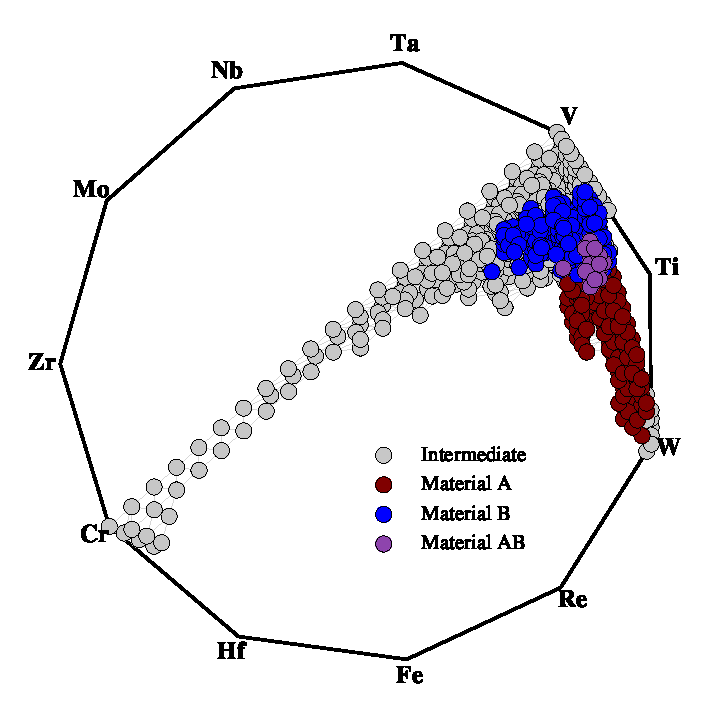
\includegraphics[width=0.75\linewidth]{figures/fig2_categories.pdf}
  \caption{Material classes of the \(686\) compositions of the design region
  (Subgraph~1), projected onto the eleven-element composition space: Material~A
  (plasma-facing, maroon), Material~B (structural, blue), Material~AB (both,
  purple), and Intermediate (neither, grey).}
  \label{fig:categories}
\end{figure}

The terminal alloys selected with \Cref{eq:ends} from the \(157\) plasma-facing (A
or AB) and \(187\) structural (B or AB) candidates are \ch{W90V5Re5}, with the
highest solidus (\(3449\)~K) and a yield strength of \(310\)~MPa at
\(600^{\circ}\)C, and \ch{W15V75Ti10}, with the highest Pugh ratio (\(3.03\)) and a
yield strength of \(285\)~MPa at \(650^{\circ}\)C. Neither terminal is a pure
element: the class definitions alone move both ends of the wall into
multicomponent alloys. Their linear CTE at \(600^{\circ}\)C, \(5.03\) and
\(9.28\times10^{-6}\)~K\(^{-1}\), sets the expansion change of
\(4.2\times10^{-6}\)~K\(^{-1}\) that the gradient must accommodate.


\subsection{Gradient Path with Monotonic CTE and Solidus}
\label{subsec:path}

A gradient that joins the two materials while satisfying every requirement exists,
and it is as short as any gradient between these terminals can be. Of the \(686\)
compositions of the design region, \(293\) are admissible layers
(\Cref{eq:admissible}), and of the \(7{,}348\) directed single-exchange steps,
\(2{,}714\) join two admissible layers and satisfy \Cref{eq:monotone}. Dijkstra's
algorithm on this graph returned a path of \(16\) steps (\(17\) alloys) from
\ch{W90V5Re5} to \ch{W15V75Ti10} (Fig.~\ref{fig:path-map}, Table~\ref{tab:path}),
verified step by step, with \(\mathrm{LOM}=0\). No path between these terminals can
be shorter, with or without monotonicity: \(75\)~at.\% W and \(5\)~at.\% Re must be
removed, \(5\)~at.\% per step. Requiring the CTE and the solidus to be monotonic at
the same time therefore adds no layers to the wall. Several paths share this
minimum length; they are equally optimal, and Dijkstra's algorithm returns one of
them deterministically.

\begin{figure}[H]
  \centering
  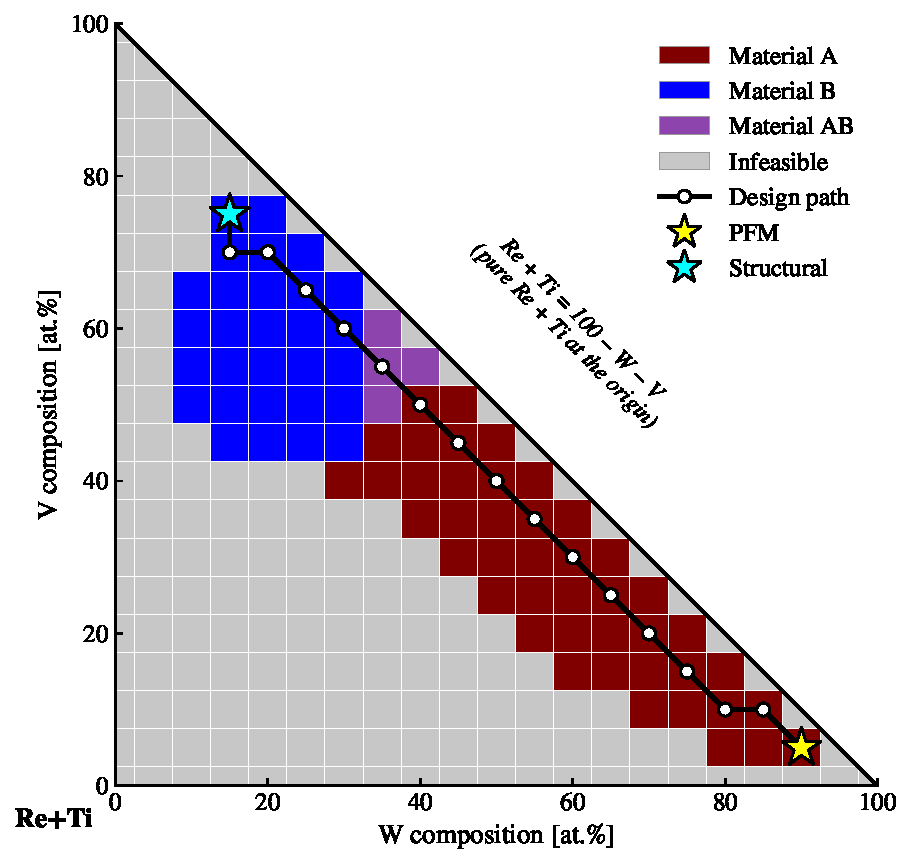
\includegraphics[width=\linewidth]{figures/fig3_design_path_map.pdf}
  \caption{The design path in W--V composition space, with the remaining path
  elements (Ti and Re) as the balance, so that the origin corresponds to pure
  Ti\(+\)Re. Each cell of the \(5\)~at.\% grid is coloured by its material class if
  it is an admissible path layer (Material~A, maroon; B, blue; AB, purple) and grey
  if any screen removes it. The path (black line, one marker per layer) runs from the
  plasma-facing terminal \ch{W90V5Re5} (yellow star) to the structural terminal
  \ch{W15V75Ti10} (cyan star).}
  \label{fig:path-map}
\end{figure}

The path divides the expansion change of the wall into sixteen small, same-signed
steps (Fig.~\ref{fig:path-profiles}). The linear CTE rises at every step, from
\(5.03\) to \(9.28\times10^{-6}\)~K\(^{-1}\) at \(600^{\circ}\)C and from \(5.06\) to
\(9.36\times10^{-6}\)~K\(^{-1}\) at \(650^{\circ}\)C, in nearly equal increments of
\(0.19\)--\(0.28\times10^{-6}\)~K\(^{-1}\). The largest step is less than a
twenty-fifth of the mismatch of about \(8\times10^{-6}\)~K\(^{-1}\) at a direct
tungsten--steel joint~\cite{fgmWsteelCGS2022}. The solidus falls at every step, from
\(3449\) to \(2262\)~K, most steeply (\(150\)--\(160\)~K per step) in the first two
tungsten-rich layers, so every layer melts at a temperature at least as high as the
layers behind it, matching the temperature drop through the wall.

\begin{figure}[H]
  \centering
  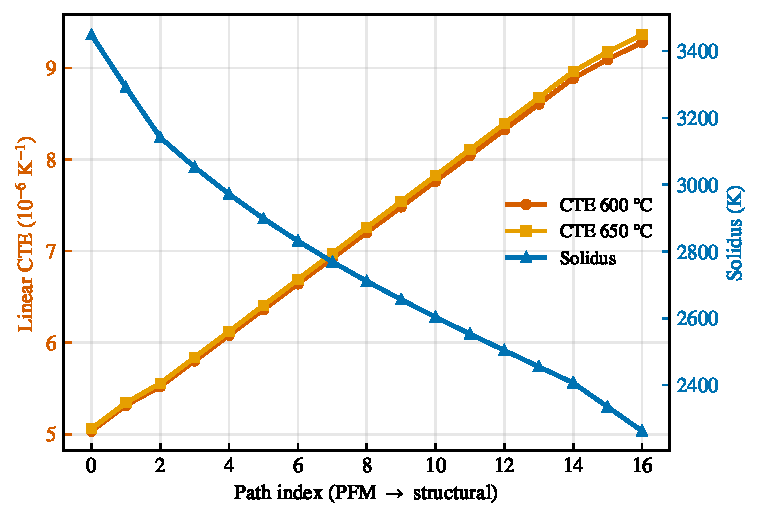
\includegraphics[width=\linewidth]{figures/fig4_cte_solidus_along_path.pdf}
  \caption{Linear CTE at \(600\) and \(650^{\circ}\)C (left axis, vermillion and
  orange) and solidus (right axis, blue) along the design path, from the plasma-facing
  terminal (path index~0) to the structural terminal (path index~16). The CTE never
  decreases and the solidus never increases from one layer to the next.}
  \label{fig:path-profiles}
\end{figure}

Properties that were not constrained along the path follow the same two-material
logic. The Pugh ratio rises from \(2.00\) to \(3.03\) without a single decrease, so
ductility increases toward the load-bearing side, because every step removes
tungsten or adds vanadium or titanium. The yield strength exceeds the EUROFER97-level
limits on every layer, with minima of \(307\)~MPa at \(600^{\circ}\)C and
\(285\)~MPa at \(650^{\circ}\)C at the two terminals and a maximum of \(824\)~MPa at
\(600^{\circ}\)C for \ch{W55V35Ti5Re5}, where W and V are most mixed, so the graded
layers are stronger than either material they join. The path passes through the
classes in order, eleven Material~A layers, two Material~AB layers, and four
Material~B layers (Table~\ref{tab:path}).

\begin{table*}[!t]
\centering
\caption{The design path: seventeen alloys connected by sixteen single
\(5\)~at.\% exchanges, from the plasma-facing terminal (layer~0) to the structural
terminal (layer~16). The linear CTE is non-decreasing at both temperatures and the solidus
non-increasing at every step; the Pugh ratio and yield strength are reported, not
constrained.}
\label{tab:path}
\begin{tabular}{cllcccccc}
\toprule
Layer & Composition (at.\%) & Step & \(T_s\) (K) & \(\alpha_{600}\) & \(\alpha_{650}\) & \(B/G\) & \(\sigma_y^{600}\) / \(\sigma_y^{650}\) (MPa) & Class \\
 & & & & \multicolumn{2}{c}{(\(10^{-6}\)~K\(^{-1}\))} & & & \\
\midrule
0  & W$_{90}$V$_{5}$Re$_{5}$         & --                  & 3449 & 5.03 & 5.06 & 2.00 & 310 / 294 & A \\
1  & W$_{85}$V$_{10}$Re$_{5}$        & W\,$-5$, V\,$+5$    & 3292 & 5.31 & 5.34 & 2.05 & 505 / 483 & A \\
2  & W$_{80}$V$_{10}$Ti$_{5}$Re$_{5}$ & W\,$-5$, Ti\,$+5$  & 3141 & 5.52 & 5.56 & 2.07 & 506 / 483 & A \\
3  & W$_{75}$V$_{15}$Ti$_{5}$Re$_{5}$ & W\,$-5$, V\,$+5$   & 3052 & 5.80 & 5.84 & 2.12 & 639 / 612 & A \\
4  & W$_{70}$V$_{20}$Ti$_{5}$Re$_{5}$ & W\,$-5$, V\,$+5$   & 2972 & 6.08 & 6.12 & 2.18 & 732 / 702 & A \\
5  & W$_{65}$V$_{25}$Ti$_{5}$Re$_{5}$ & W\,$-5$, V\,$+5$   & 2898 & 6.36 & 6.41 & 2.24 & 791 / 758 & A \\
6  & W$_{60}$V$_{30}$Ti$_{5}$Re$_{5}$ & W\,$-5$, V\,$+5$   & 2831 & 6.64 & 6.69 & 2.30 & 820 / 786 & A \\
7  & W$_{55}$V$_{35}$Ti$_{5}$Re$_{5}$ & W\,$-5$, V\,$+5$   & 2769 & 6.92 & 6.97 & 2.36 & 824 / 789 & A \\
8  & W$_{50}$V$_{40}$Ti$_{5}$Re$_{5}$ & W\,$-5$, V\,$+5$   & 2711 & 7.20 & 7.26 & 2.43 & 804 / 769 & A \\
9  & W$_{45}$V$_{45}$Ti$_{5}$Re$_{5}$ & W\,$-5$, V\,$+5$   & 2656 & 7.48 & 7.54 & 2.50 & 765 / 730 & A \\
10 & W$_{40}$V$_{50}$Ti$_{5}$Re$_{5}$ & W\,$-5$, V\,$+5$   & 2603 & 7.76 & 7.83 & 2.57 & 709 / 675 & A \\
11 & W$_{35}$V$_{55}$Ti$_{5}$Re$_{5}$ & W\,$-5$, V\,$+5$   & 2553 & 8.04 & 8.11 & 2.65 & 638 / 606 & AB \\
12 & W$_{30}$V$_{60}$Ti$_{5}$Re$_{5}$ & W\,$-5$, V\,$+5$   & 2503 & 8.32 & 8.39 & 2.73 & 557 / 526 & AB \\
13 & W$_{25}$V$_{65}$Ti$_{5}$Re$_{5}$ & W\,$-5$, V\,$+5$   & 2455 & 8.60 & 8.68 & 2.82 & 467 / 439 & B \\
14 & W$_{20}$V$_{70}$Ti$_{5}$Re$_{5}$ & W\,$-5$, V\,$+5$   & 2406 & 8.89 & 8.96 & 2.91 & 373 / 349 & B \\
15 & W$_{15}$V$_{70}$Ti$_{10}$Re$_{5}$ & W\,$-5$, Ti\,$+5$ & 2334 & 9.09 & 9.17 & 2.96 & 342 / 319 & B \\
16 & W$_{15}$V$_{75}$Ti$_{10}$        & Re\,$-5$, V\,$+5$  & 2262 & 9.28 & 9.36 & 3.03 & 307 / 285 & B \\
\bottomrule
\end{tabular}
\end{table*}

The path is also simple to build (Fig.~\ref{fig:path-composition}). Although it was
planned in an eleven-element space, it uses only W, V, Ti, and Re: tungsten falls
from \(90\) to \(15\)~at.\% as vanadium rises from \(5\) to \(75\)~at.\%, titanium
enters at \(5\)~at.\% in the second step and rises to \(10\)~at.\% near the
structural end, and rhenium stays at \(5\)~at.\% until the final step. The gradient
can thus be deposited mainly by varying the W and V feeds, with the Ti and Re
additions changed only three times. Iron is absent from every layer, so the
tungsten--iron intermetallics that limit conventional tungsten-to-steel gradients
cannot form anywhere along the wall.

\begin{figure}[H]
  \centering
  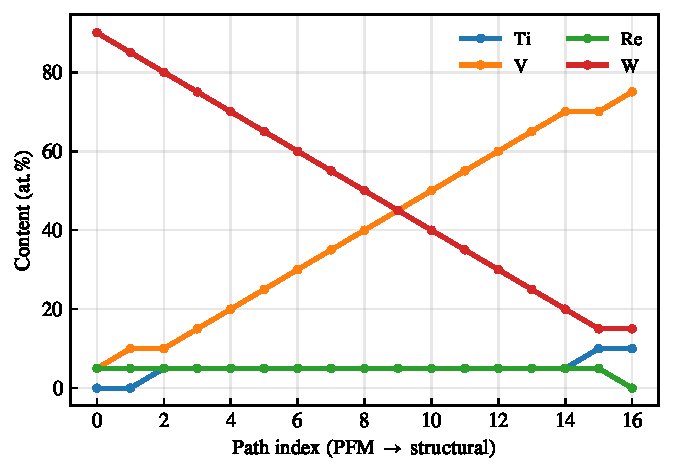
\includegraphics[width=0.9\linewidth]{figures/fig5_composition_profile.pdf}
  \caption{Composition of W, V, Ti, and Re along the design path, from the
  plasma-facing terminal (path index~0) to the structural terminal (path
  index~16). Each step exchanges \(5\)~at.\% of one element for another: a W--V
  gradient with Ti added at layers~2 and~15 and Re removed at the final layer.}
  \label{fig:path-composition}
\end{figure}

Together, these results show that the two materials of the first wall can be joined
by a single-phase, reduced-activation gradient in which every requirement holds
layer by layer, and that the two monotonicity requirements cost nothing in the
number of layers. Two limitations apply. First, the properties are model estimates,
the yield strength from the Maresca--Curtin model, the Pugh ratio from a rule of
mixtures, and the solidus and CTE from CALPHAD; they are suited to ranking
compositions and setting the direction of the gradient, but the values along the
path, in particular for the vanadium-rich layers, should be confirmed by measurement
on the terminal alloys and selected intermediate layers before the gradient is
built. Second, the path ensures that the CTE changes in one direction only, but the
thermal stresses in the graded wall were not computed; such an analysis requires
the layer thicknesses and the through-wall temperature field and was considered
outside the scope of this work, as it would not change the path design methodology.
